%The computational model of Lazy Shadowing has been continuously optimized to improve its scalability and efficiency, to eliminate vulnerability, and to reduce implementation complexity and overhead. This section presents the system design of Rejuvenating Shadows. 

%\subsection{Fault model}

We adopt the fail-stop fault model, which defines that a process halts in response to a failure and its internal state and memory contents are irretrievably 
lost~\cite{Schlichting1983}. Furthermore, we assume that the machine on which failure occurred can be rebooted for starting a new process after the failure. Note that this is the same assumption for checkpointing/restart. Below we discuss the components of the Rejuvenating Shadows model and its design trade-offs.
 
%As demonstrated in~\cite{cui_2016_scalcom}, Lazy Shadowing is able to tolerate both hardware and software failures under the fail-stop fault model. In this work, we continue with the assumption of fail-stop model. In order to further improve resilience and efficiency, however, Rejuvenating Shadows differentiates between temporary failures and permanent failures. Temporary failures include memory bit flips, kernel panic, etc., and can be recoverd by rebooting the machine, while permanent failures, such as failure in power supply and network switch, needs the device to be replaced in order to recover. Rejuvenating Shadows maximizes the resource utilization for resilience by adopting different strategies for different types of failures. 

\subsection{Shadowing}
\label{sec:shadow}
The basic tenet of Shadowing is to associate with each process (referred to as main) a replica process (referred to as shadow), which potentially runs at a lower execution rate to save power and computing resources. Originally, if a main fails, its shadow is promoted to assume the role of the main. 
%In this way, shadow processes are substitutes for mains in the case of failure. 
In this work, however, we deviate from the original concept of shadow as a replica~\cite{cui_2016_scalcom} and use the state of the shadow to restore the main to its state prior to the failure. 

%\subsection{Consistency}
%\label{sec:consistency}

State consistency between mains and shadows is required both during normal execution and following a failure. % of a main process to roll-forward the shadows. 
As depicted in Figure~\ref{fig:cons_protocol}, we designed a protocol
to enforce sequential consistency, i.e., each shadow sees the same message order and operation results as its main. 
%In this figure, A and B represent two mains, and A' and B' are their shadows. 
Instead of sending messages from main to main and shadow to shadow~\cite{ferreira_sc_2011}, we choose to let the sending main forward each message to the receiving shadow. This allows us to speed up a single shadow when a main fails. 
%For each message, the sending main sends a copy of the message to both the receiving main and its shadow, and the shadow of the sender is suppressed from sending out messages. 
We assume that two copies of the same message are sent in an atomic manner.\footnote{this property can be ensured, for example, by using the NIC multicast functionality of the network.}
Note that, the SYNC message in Figure~\ref{fig:cons_protocol} is only used to address potential non-determinism as will be discussed in details in the next section.


\begin{figure}[!t]
  \begin{center}
      	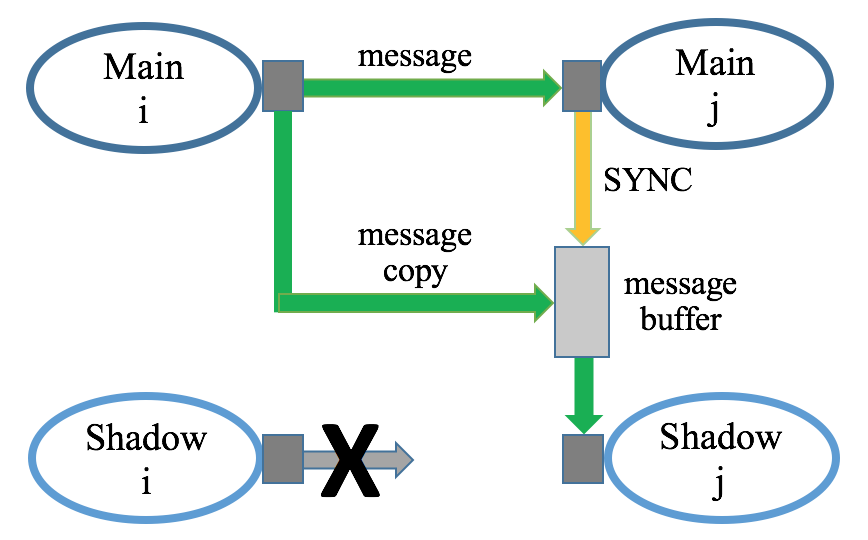
\includegraphics[width=0.7\columnwidth]{figures/consistency}
  \end{center}
  \vskip -0.2in
  \caption{Consistency protocol for Rejuvenating Shadows.}
  \label{fig:cons_protocol}
\end{figure}

%The SYNC message in Figure~\ref{fig:cons_protocol} is only used when there is potential non-determinism. This will be discussed in details in the next Section.
%We assume that only MPI operations can introduce non-determinism. MPI\_ANY\_SOURCE may result in different message receiving orders between a main and its shadow. To deal with this, we serialize MPI\_ANY\_SOURCE message receiving by having the main first do the receiving and then use a SYNC message to forward the message source information to its shadow, which then issues a receiving with the specific source. Other operations, such as MPI\_Wtime() and MPI\_Probe(), can be dealt with in a similar manner by forwarding the result from a main to its shadow.

To reduce the execution rate of the shadows, one can use Dynamic Voltage and Frequency Scaling (DVFS)~\cite{cui_en7085151}, process collocation~\cite{cui_2016_scalcom}, or a combination of both. Because of the undesirable consequences entailed by DVFS, such as reduced reliability and limited control granularity, we choose to use only collocation in this work. %The implementation details are presented in Section~\ref{sec:rate_control}. 
Collocation increases memory requirement for the nodes that execute shadows. Note that, however, this problem is not intrinsic to Rejuvenating Shadows, as in-memory and multi-level checkpointing also require extra memory.
The number of shadows collocated on a processing unit is referred to as the \textit{collocation ratio}. Also, the term \textit{shadowed set} is used to refer to a set of mains and their associated shadows of which the shadows are collocated. Figure~\ref{fig:logical_org} shows an example of three shadowed sets with collocation ratio of 4.

\begin{figure}[!t]
  \begin{center}
      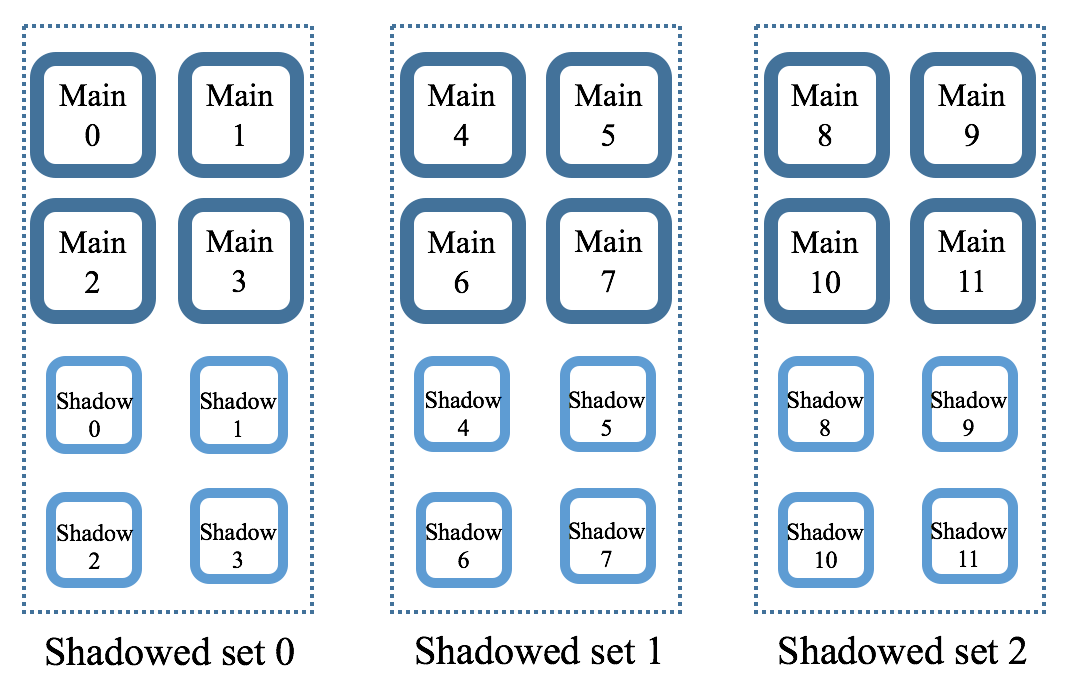
\includegraphics[width=\columnwidth]{figures/logical_org_3}
  \end{center}
  \vskip -0.25in
  \caption{Logical organization of 12 mains and their shadows with every 4 shadows collocated, resulting in 3 shadowed sets.}
  \label{fig:logical_org}
  \vskip -0.25in
\end{figure}

\subsection{Leaping}

%Leaping was initially proposed as a technique to boost the performance of lazy shadows~\cite{cui_2016_scalcom}. 
Since shadows execute slower than mains, recovery of a main failure requires a shadow to catch up, thus introduces delay to the execution. To mitigate this issue, we propose a technique, referred to as \textit{Leaping}, that takes advantage of the recovery time to synchronize the state of the shadows with that of their non-faulty mains. As a result, shadows achieve forward progress with minimal overhead, and furthermore, the recovery time of future failures, if any, is minimized. 
Leaping always takes between a pair of main and shadow. To avoid ambiguity, the process which provides state in a leaping is referred to as the target process, and the other process which receives and updates state is referred to as the roll forward process. 


%With rejuvenation, we furter extend the concept of leaping to restore a failed process using the state of its associated process. In both cases, leaping takes between a pair of main and shadow. To avoid ambiguity, the process which provides state in a leaping is referred to as the target process, and the other process which receives and updates state is referred to as the roll forward process. 

%Recently, we have identified an empirical problem to which leaping is a solution. When Lazy Shadowing is used to execute an MPI application, application messages are generated at the rate of the mains, but consumed by the shadows at a lower rate because the shadows are slower. As a result, messages accumulate on the shadow side and could possibly result in a buffer overflow. Leaping is naturally a solution to this problem as it can move the shadows forward and synchronize their execution states with those of the mains. After the synchronization, accumulated messages at the shadows become obsolete and thus can be safely discarded. To differentiate the two cases where leaping is used, leaping during failure recovery is referred to as failure induced leaping while leaping to avoid buffer overflow is referred to as forced leaping. 

\subsection{Rejuvenation}


Lazy Shadowing assumes that when a main fails, its shadow increases its execution rate to speed up recovery. %In the case where the collocation ratio is greater than one, 
With collocation, this is accomplished by terminating the other collocated shadows. As a result, however, only one instance of each task in the shadowed set remains, %. A subsequent fault in any task of this shadowed set will cause a system failure, 
thereby making the shadow set vulnerable to future faults.

%Lazy Shadowing assumes that at most one failure will occur to a pair of main and shadow. If a process fails, only one instance of the corresponding task is left. Consequently, the vulnerability of the system increases as failure increases. Collocation of shadows further exacerbates this problem, as the promotion of a shadow to a new main requires the termination of all collocated processes, so that the new main can speed up to the rate of other mains. As a result, each shadowed set can only tolerate one failure. After the first failure, all main processes in the shadowed set would lose their shadows and become vulnerable.

%It has been discussed in ~\cite{cui_2016_scalcom} that each shadowed set can only tolerate one failure. After the first failure, all main processes in the shadowed set would lose their shadows and become vulnerable. Although quantitative study show that a second failure in a shadowed set is unlikely, % even with over one million processes, 
%in practice the system will become more and more vulnerable as failures occur. In many cases, it is too costly to take such risk, especially for long-running, large-scale, and mission-critical applications. Therefore, it is preferable to maintain the same level of resilience at all times.

The shadow set vulnerability can be avoided by using rejuvenation, whereby a new process is spawned for either a failed man or shadow. This eliminates the need for a shadow to permanently substitute for a main. As result, collocated shadows need not to be terminated, but only temporarily suspended during the recovery process.  %Upon recovery, every main is always guaranteed to have an associated shadow. The problem, however, is that the newly spawned process will start from its initial state and may lag far behind the other processes. When the new process needs to synchronize with other processes, significant delay will be incurred as a result of the lag. 

The problem, however, is that the newly spawned process will start from its initial state and potentially delay the entire execution.
%Leaping provides the solution, with minimum overhead, 
To deal with this issue, we extend the concept of leaping to synchronize the new process' state with the state of its associated living process. We ignore the case where both the main and shadow of a task fail simultaneously, due to the extremely low probability. If necessary, however, the shadow replication model is always able to achieve higher reliability with the cost of more shadows per task. 


%Consider a pair of main process, $M$, and shadow process, $S$, for example. If $M$ fails, a new main process will be started to replace $M$, and then a leaping from $S$ will advance the new process to the state of $S$. This is illustrated in Figure~\ref{fig:faulty}. 
Figure~\ref{fig:rejuvenation} illustrates the failure recovery process with rejuvenation, assuming that a main $M_i$ fails at time $T_0$.
In order for its shadow $S_i$ to speed up, the shadows collocated with $S_i$ are temporarily suspended. %, so that $S_i$ can increase its execution rate and finish the recovery as soon as possible. 
Meanwhile, the failed processor is rebooted and then a new process is launched for $M_i$. When, at $T_1$, $S_i$ catches up with the state of $M_i$ before its failure, leaping is performed to advance the new process to the current state of $S_i$. The leaping is not initiated until $S_i$ catches up so as to avoid the need of message logging. 

Because of the failure of $M_i$, the other mains are blocked at the next synchronization point, which is assumed to be immediately after $T_0$. During the idle time, a leaping is opportunistically performed to transfer state from each living main to its shadow. Therefore, this leaping has minimal overhead as it overlaps with the recovery, as shown in Figure~\ref{fig:non_faulty_diff}. Figure~\ref{fig:non_faulty_same} shows that leaping for the shadows collocated with $S_i$ are delayed until the recovery completes at $T_1$. After the leaping finishes at $T_2$, all mains and shadow resume normal execution with the same level of resilience as before the failure.

Figure~\ref{fig:rejuvenation} and the above analysis assume that the time for rebooting is no longer than the recovery time. If the new $M_i$ is not yet ready when $S_i$ catches up at $T_1$, however, we have two design choices: 1) $S_i$ can continue execution and take the role of a main; or 2) $S_i$ can wait for the new $M_i$ to launch. The first option requires all the other processes to update their internal process mapping in order to correctly receive messages from this shadow (see Figure~\ref{fig:cons_protocol}). This not only complicates the implementation, but also requires expensive global coordination that is detrimental to scalability. We therefore chose the second design option.


%On the other hand, if $S$ fails, a new shadow process will be started and immediately advanced to the state of $M$ by leaping.

\begin{figure}[!t]
	\begin{center}
		\subfigure[Faulty task]
		{
			\label{fig:faulty}
			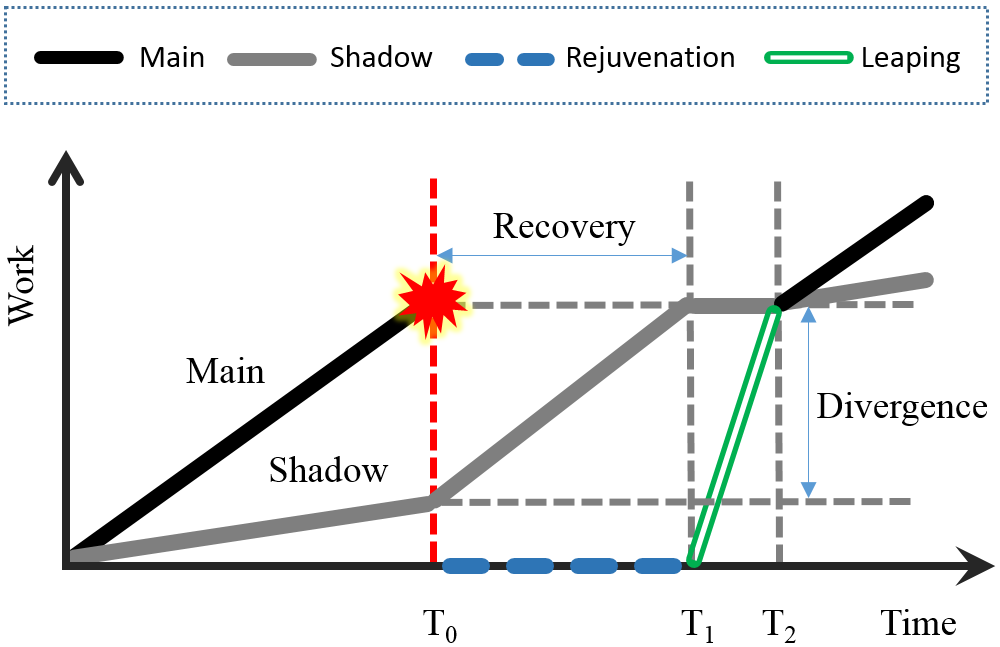
\includegraphics[width=0.7\columnwidth]{figures/rs1}
		}
		\subfigure[Non-faulty tasks in different shadowed sets]
		{
			\label{fig:non_faulty_diff}
			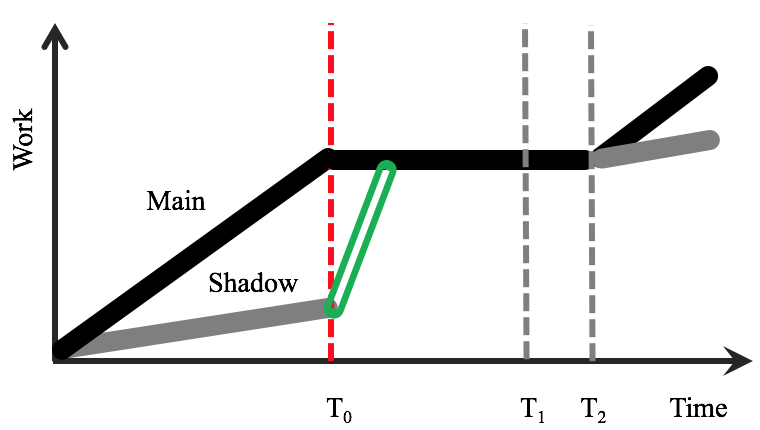
\includegraphics[width=0.7\columnwidth]{figures/rs2}
		}
		\subfigure[Non-faulty tasks in the same shadowed set]
		{
			\label{fig:non_faulty_same}
			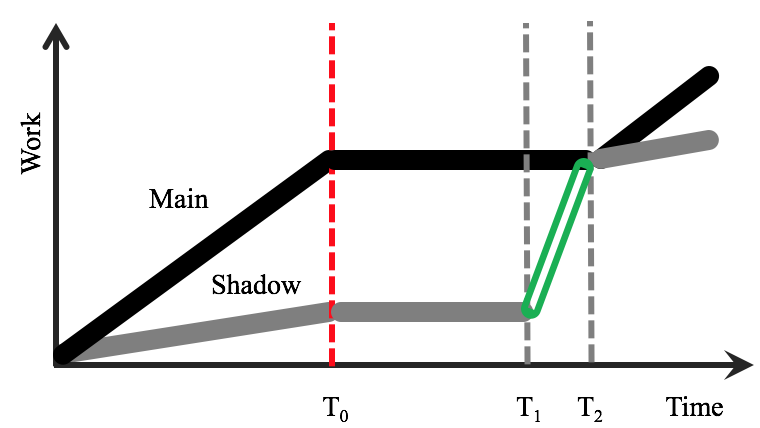
\includegraphics[width=0.7\columnwidth]{figures/rs3}
		}
	\end{center}
	\vskip -0.2in
	\caption{Recovery and rejuvenation after a main process fails.}
	\label{fig:rejuvenation}
\end{figure}

%Depending on the type of failure, the new process will be placed at different locations. If it is a temporary failure, the node where failure occurs will be rebooted and then used to host the new process, whether it is a main or shadow. Although there is a delay from the rebooting, it is usually small compared to application's running time and can be accounted part of the recovery. 
%For permanent failures, the node cannot be used and we have to migrate and collocate some processes. If the new process is a main, its existing shadow will be migrated to another node where shadow process(es) reside, and make room for the new main. Otherwise, if the new process is a shadow, it will be directly created on a shadow node. 
